\begin{enumerate}
\item De ce que l'on voit de la courbe, la fonction est manifestement convexe d'abord, puis concave. Comme la tangente à $\mathcal{C}_f$ au point A semble traverser la courbe au point de tangence, on peut émettre la conjecture que la fonction $f$ est convexe sur $]-\infty~;~1]$ et concave sur $[1~;~+\infty[$.
\item On a :
\quad $ \begin{cases} \lim\limits_{x \to -\infty } x^2+1 = +\infty \\
\lim\limits_{X \to +\infty } \ln(X) = +\infty \end{cases} $\quad donc, par composition, \quad $ \lim\limits_{x \to -\infty} \ln (x^2+1) = +\infty$.

De plus, \quad $\lim\limits_{x \to -\infty} -3x = +\infty$

Donc par produit et somme, \quad $\lim\limits_{x \to -\infty} f(x) = +\infty$.
\item 
	\begin{enumerate}
		\item Soit $x$ un réel strictement positif.

$\begin{aligned} f(x) &= 5 \ln \left(x^{2}+1\right)-3 x\\
	&= 5 \ln \left(x^{2} \left(1 + \dfrac{1}{x^2}\right)\right)-3 x \\
	&= 5\ln \left(x^2 \right) + 5 \ln \left(1+\dfrac{1}{x^{2}}\right) -3x\quad \text{par propriété de la fonction ln}.\\
	&= 5 \times 2 \ln(x) -3x + 5 \ln \left(1+\dfrac{1}{x^{2}}\right) \\
	&= x\left(10 \dfrac{\ln x}{x}-3\right)+5 \ln \left(1+\dfrac{1}{x^{2}}\right)
\end{aligned}$

On a donc bien : pour tout $x$ réel strictement positif,\quad $f(x)=x\left(10 \dfrac{\ln x}{x}-3\right)+5 \ln \left(1+\dfrac{1}{x^{2}}\right)$.
		\item On va utiliser la forme établie à la question précédente pour lever l'indétermination :
		\begin{itemize}
			\item D'une part :

D'après la propriété des croissances comparées,\quad $\lim\limits_{x\to +\infty} \dfrac{\ln(x)}{x} = 0$.

Donc par produit et somme,\quad $ \lim\limits_{x\to +\infty} 10\dfrac{\ln(x)}{x} - 3= - 3$.

De plus \quad $\lim\limits_{x \to +\infty } x = +\infty $ \quad donc par produit, \quad $\lim\limits_{x \to +\infty } x\left(10 \dfrac{\ln x}{x}- 3\right) = -\infty$.

			\item D'autre part :
\quad
$ \begin{cases} \lim\limits_{x \to +\infty } 1 + \dfrac{1}{x^2} = 1 \\
\lim\limits_{X \to 1} \ln(X) = 0 \end{cases} $ \quad par composition, \quad $ \lim\limits_{x \to +\infty} \ln \left(1+\dfrac{1}{x^{2}}\right) = 0$

Par produit on a donc $ \lim\limits_{x \to +\infty} 5 \ln \left(1+\dfrac{1}{x^{2}}\right) = 0$.
		\end{itemize}

		Finalement, par somme,\quad $\lim\limits_{x \to +\infty} f(x) = -\infty$.
\end{enumerate}
\item
	\begin{enumerate}
		\item Pour déterminer l'expression de la fonction dérivée de $f$, on va revenir à l'expression de départ de $f(x)$, plus simple que celle obtenue à la question \textbf{3. a.}.

On a admis que $f$ est dérivable sur $\R$.

Si on pose :\quad $\begin{cases}u : x \longmapsto x^2 + 1\\ u' : x \longmapsto 2x \end{cases}$ \quad on a \quad $\forall x \in \R,\quad f(x) = 5\ln\big(u(x)\big) - 3x$.

Ainsi, on a :\quad $\forall x \in \R,\quad \begin{aligned}[t]
	f'(x) &= 5\dfrac{u'(x)}{u(x)}-3\\
	&=2\dfrac{2x}{x^2 + 1} - 3\\
	&=\dfrac{10x}{x^2 + 1} + \dfrac{-3\big(x^2 + 1\big)}{x^2 + 1}\\
	&=\dfrac{10x -3x^2 - 3}{x^2 + 1}\\
	&=\dfrac{-3x^2 + 10x - 3}{x^2 + 1}\\
\end{aligned}$

On arrive bien à l'expression attendue.

\item Pour tout $x$ réel, l'expression \quad $x^2 + 1$ \quad est supérieure à 1, et donc strictement positive.

Le signe de $f'(x)$ est donc celui du trinôme :\quad $-3x^2 + 10x - 3$.

Ce trinôme a un coefficient dominant égal à $-3$, donc négatif. Cela signifie que toutes les images \quad $-3x^2 + 10x - 3$ \quad sont négatives, sauf pour les valeurs $x$ comprises entre d'éventuelles racines.

Le discriminant du trinôme est :\quad $\Delta = 10^2 - 4\times (-3) \times (-3) = 100 - 36 = 64 = 8^2$.

Comme il est strictement positif, le trinôme admet deux racines réelles distinctes :

$x_1 = \dfrac{-10 - 8}{2\times (-3)} = 3$\quad et \quad  $x_2 = \dfrac{-10 + 8}{2\times (-3)} = \dfrac{1}{3}$.

On peut donc établir le tableau de signe suivant :

\hfill~\begin{tikzpicture}
\tkzTabInit[lgt=4,espcl=2]{$x$/1.1, signe de $-3x^2 + 10x - 3$/1,signe de $f'(x)$/1}
{$-\infty$,$\dfrac{1}{3}$,$3$,$+\infty$}
\tkzTabLine{,-,z,+,z,-,}
\tkzTabLine{,-,z,+,z,-,}
\end{tikzpicture}\hfill~

On a donc une fonction $f$ qui est strictement décroissante sur l'intervalle $\left]-\infty ; \dfrac{1}{3}\right]$, ainsi que sur l'intervalle $[3 ; +\infty[$ et strictement croissante sur l'intervalle $\left[\dfrac{1}{3} ; 3\right] $.

Ceci est cohérent avec la courbe tracée sur le sujet.
		\end{enumerate}
\item 
	\begin{enumerate}
		\item Puisque l'expression de la fonction dérivée seconde est donnée, on va pouvoir utiliser ce résultat.

Le dénominateur \quad $\big(x^2 + 1\big)^2$\quad est à valeurs strictement positives sur $\R$, en tant que carré d'un réel lui-même strictement positif.

$f''(x)$ a donc le même signe que son numérateur :\quad $-10x^2 + 10 = 10(1 - x^2) = 10(1 - x)(1 + x)$.

Le numérateur est donc une expression polynomiale de degré 2, dont le coefficient dominant est négatif, et ayant deux racines évidentes : 1 et $-1$.

On peut donc établir le tableau de signe de $f''(x)$ :

\hfill~\begin{tikzpicture}
\tkzTabInit[lgt=4,espcl=2]{$x$/0.7, signe de $f''(x)$/0.7}
	{$-\infty$,$-1$,$1$,$+\infty$}
	\tkzTabLine{,-,z,+,z,-,}
\end{tikzpicture}\hfill~

$f$ est donc convexe sur $[-1 ; 1]$, et concave sur $]-\infty ; -1]$ ainsi que sur $[1 ; +\infty[$, avec deux points d'inflexion, à l'abscisse $-1$ et à l'abscisse 1(c'est le point A).

Cela permet donc de rejeter la conjecture formulée à la question \textbf{1.}. Cette conjecture est faussée par l'échelle choisie pour la représentation de $f$. Ci-après, avec une échelle qui permet d'observer les images pour des abscisses inférieures à 1, la concavité de cette zone devient apparente :

\hfill~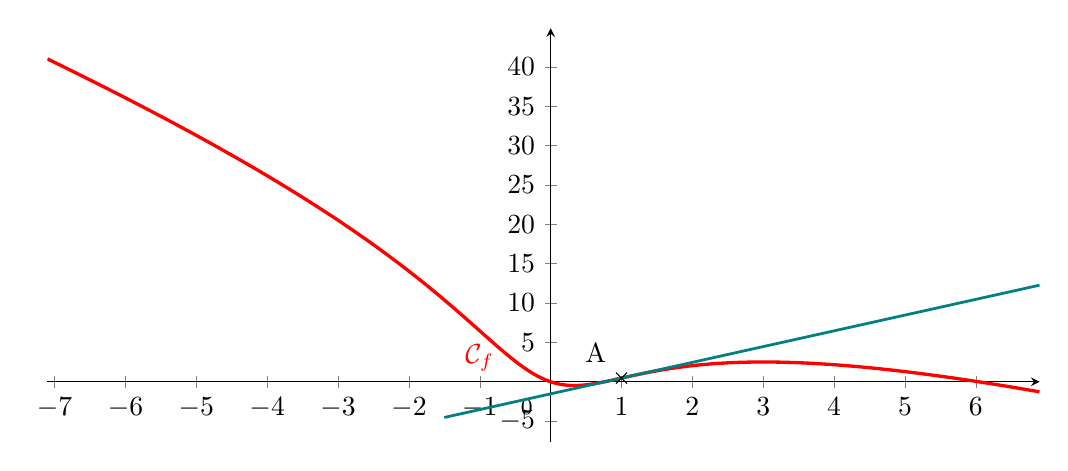
\begin{tikzpicture}[baseline={(current bounding box.center)}]
	\begin{axis}[
	x={9mm}, y={1mm},
	xmin = -7.1, xmax = 6.9,
	ymin = -7.7, ymax = 44.9,
	xtick distance=1,
	ytick distance=5,
	minor tick num = 0,
	grid=none, axis lines =center]
	\node[below left=3pt] at (axis cs: 0,0) {{\footnotesize 0}};
	\addplot [line width=1.2pt, color=red, smooth, samples=100, domain= -7.1:6.9 ]{5*ln(x*x+1)-3*x};
	\node[red] at(axis cs: -1,3) {$\mathcal{C}_f$};
	\addplot [line width=1pt, color=teal, smooth, samples=10, domain= -1.5:6.9 ]{2*x-1.534};
	\draw[shift={(axis cs: 1,0.466)}] (-2pt,-2pt)--(2pt,2pt) (-2pt,2pt)node[above left]{A}--(2pt,-2pt) ;
\end{axis}
\end{tikzpicture}\hfill~

	\item L'équation réduite de la tangente à la courbe $\mathcal{C}_{f}$ au point A d'abscisse 1 est donnée par la formule classique :
\quad $y = f'(1) \times \big(x - 1\big) + f(1)$.

Avec : \quad $f(1) = 5\ln(1^2 + 1) - 3\times 1 = 5\ln(2) - 3$;

et : \quad $f'(1) = \dfrac{-3\times 1^2 + 10 \times 1 - 3}{1^2 + 1} = \dfrac{4}{2} = 2$;

On arrive à :\quad $y = 2\big(x - 1\big) + 5\ln(2) - 3$\quad soit  \quad $y = 2x + 5\ln(2) - 5$.

	\item On nous demande d'établir une inégalité pour $x \geqslant 1$.

Sur $[1~;~+\infty[$, on a établi à la question \textbf{5. a.} que la fonction est concave.

Graphiquement, cela se traduit par le fait que la courbe représentative de $f$ est en dessous de toutes ses tangentes sur cet intervalle, notamment en dessous de celle au point d'abscisse 1, dont on vient de déterminer l'équation.

On peut donc affirmer :\quad $\begin{aligned}[t]
	f(x) \leqslant 2x + 5\ln(2) - 5
	&\iff 5\ln\big(x^2 + 1\big) - 3x \leqslant 2x + 5\ln(2) - 5\\
	&\iff 5\ln\big(x^2 + 1\big) \leqslant 3x + 2x + 5\ln(2) - 5\\
	&\iff 5\ln\big(x^2 + 1\big) \leqslant 5x + 5\ln(2) - 5\\
	&\iff 5\ln\big(x^2 + 1\big) \leqslant 5\big(x + \ln(2) - 1\big)\\
	&\iff \ln\big(x^2 + 1\big) \leqslant x + \ln(2) - 1\quad \text{ car } 5 > 0\\
\end{aligned}$

On établit donc ainsi l'inégalité demandée.
	\end{enumerate}
\end{enumerate}
